\section{Methods}
\begin{frame}{Motivation and methods overview}
    
   \begin{block}{Motivation}
       To obtain model parameter margins and to assess model sensitivity to provide usability limits and parameter sets for potential users.
   \end{block}
   \bigskip
   \begin{block}{Methods}
       \begin{enumerate} 
           \item Use data ensemble to optimize model parameters 
           \item Store parameters of all ``good" runs for each measurement
           \item Explore results of the ``best" models
           \item Explore distribution parameters of ``best" models
       \end{enumerate} 
   \end{block}

   
\end{frame}


    \begin{frame}{Use data ensemble to optimize model parameters}
    \medskip
    Data ensemble: 
    \begin{itemize}
       \item 55 plot scale, laboratory artificial rainfall experiments, several locations
       \item sheet velocity, specific discharge
    \end{itemize}

    Parameters:
    \begin{itemize}
       \item Philips infiltration: $K_s$, $S$
       \item Shallow water surface flow: $X$, $Y$, $b$
       \begin{itemize}
           \item $v = Xi^Yh^b$
       \end{itemize}
       \item surface retention
    \end{itemize}

    Optimization:
    \begin{itemize}
       \item Differential evolution, storing all the intermediate results
       \item Two variables optimized: water level $h$, specific discharge $q$
       \item Sum of squares as objective function (NS also calculated)
    \end{itemize}



\end{frame}

\begin{frame}{Use data ensemble to optimize model parameters}
   Example of single optimized measurement. 
   \begin{center}
   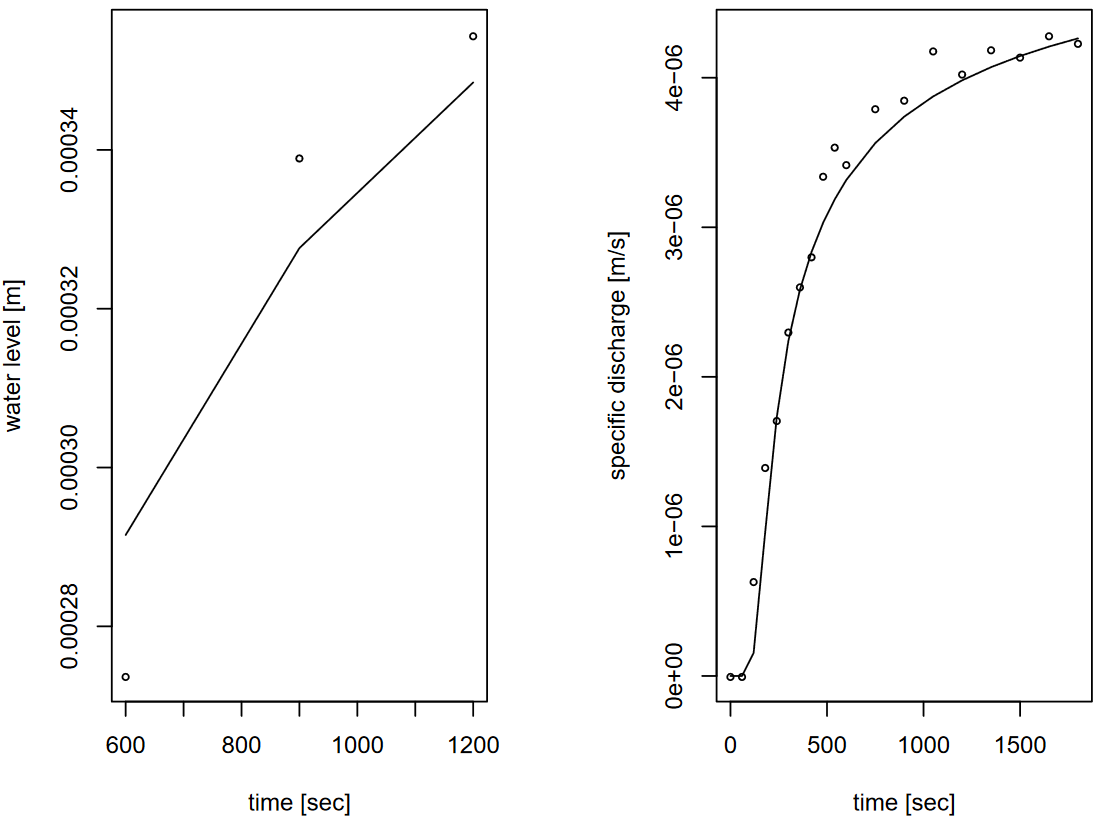
\includegraphics[width=0.6\paperwidth]{img/optim}
   \end{center}
\end{frame}





\begin{frame}{Store parameters of all ``good" runs for each measurement}
\begin{columns}
   \begin{column}{0.4\linewidth}
   Select model runs with:\\ (NS($h$) and NS($q$)) $>$ 0\\
   \bigskip
   Make a Pareto front at \\ the SS($h$) and SS($q$) scatter plot
   \end{column}
   \begin{column}{0.6\linewidth}
   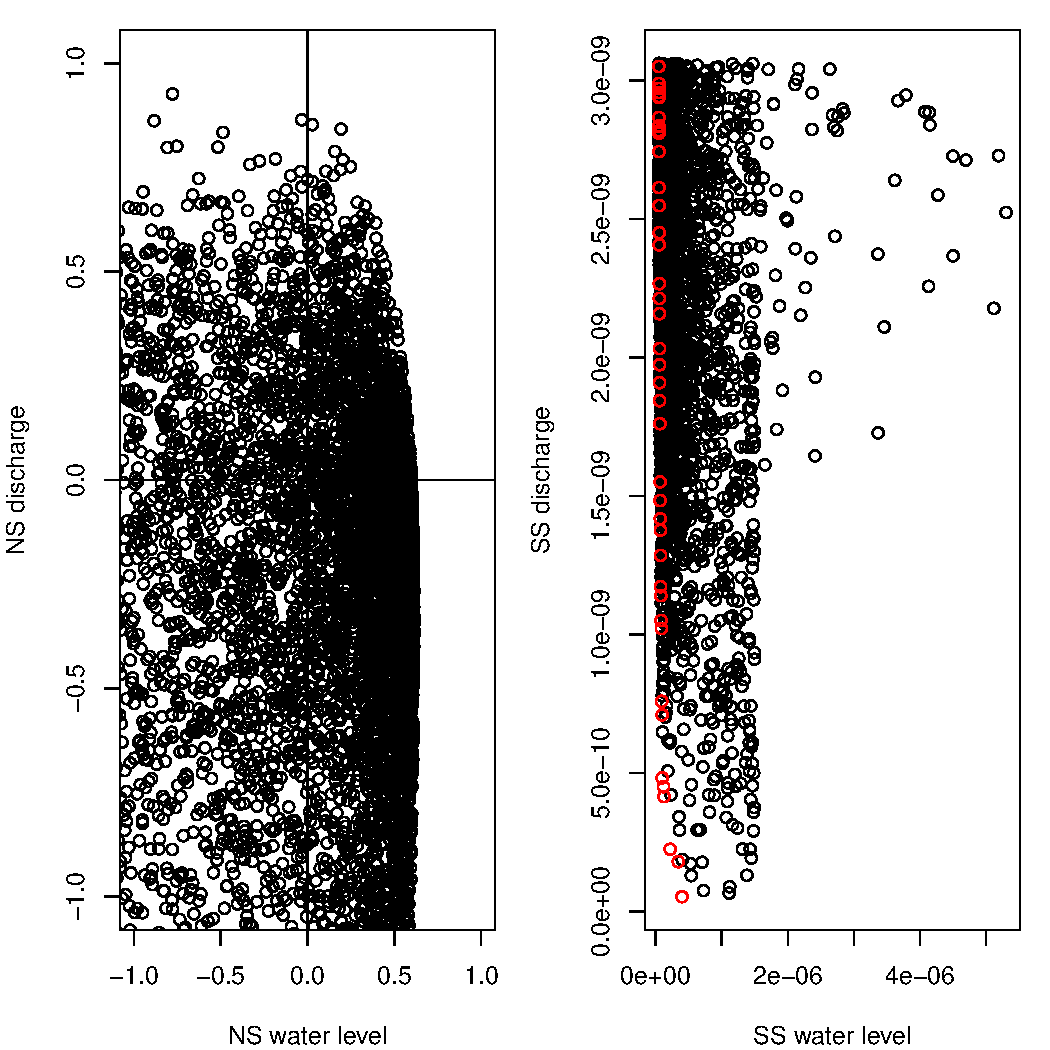
\includegraphics[width=0.9\linewidth]{img/pareto}
   \end{column}
\end{columns}

\end{frame}

\begin{frame}{Explore results of the ``best" models (in progress...)}
   Specific discharge is less sensitive compared to flow velocity. Specific discharge is almost not sensitive to the parameters $X$, $Y$, $b$.
   \begin{center}
   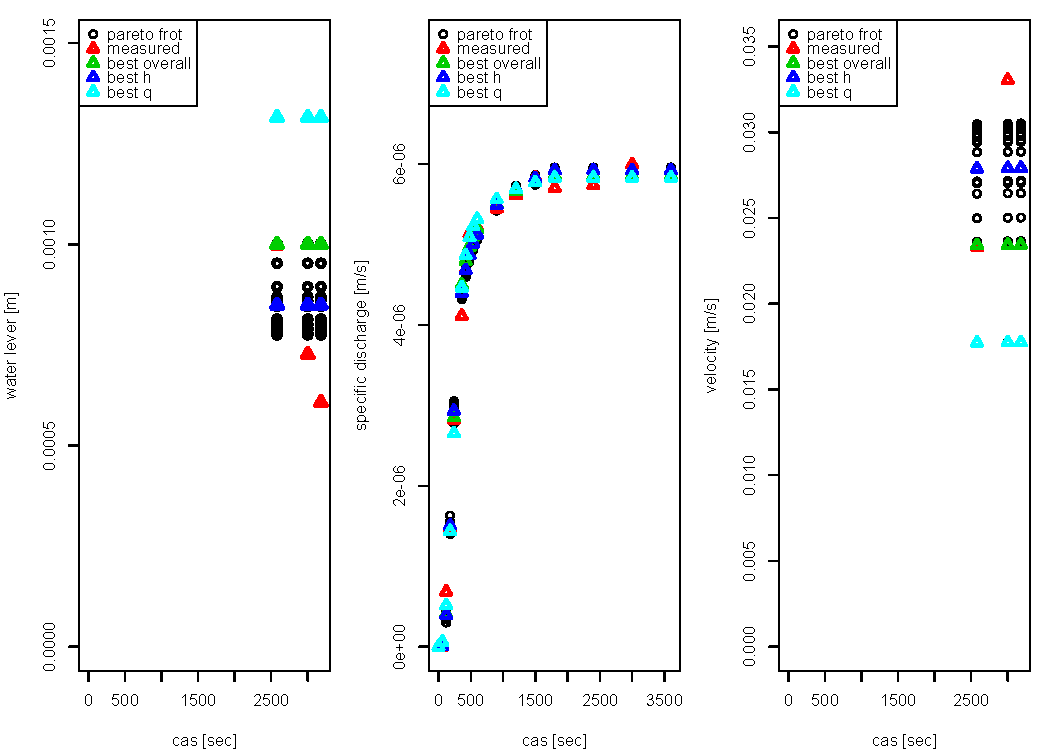
\includegraphics[width=0.6\paperwidth]{img/priklad}
   \end{center}
\end{frame}


\begin{frame}{Explore distribution parameters of ``best" models (in progress...)}
   All parameters but $X$ and $b$ exhibited unimodal distribution. $X$ is likely sensitive to current soil surface conditions. 
   \begin{center}
   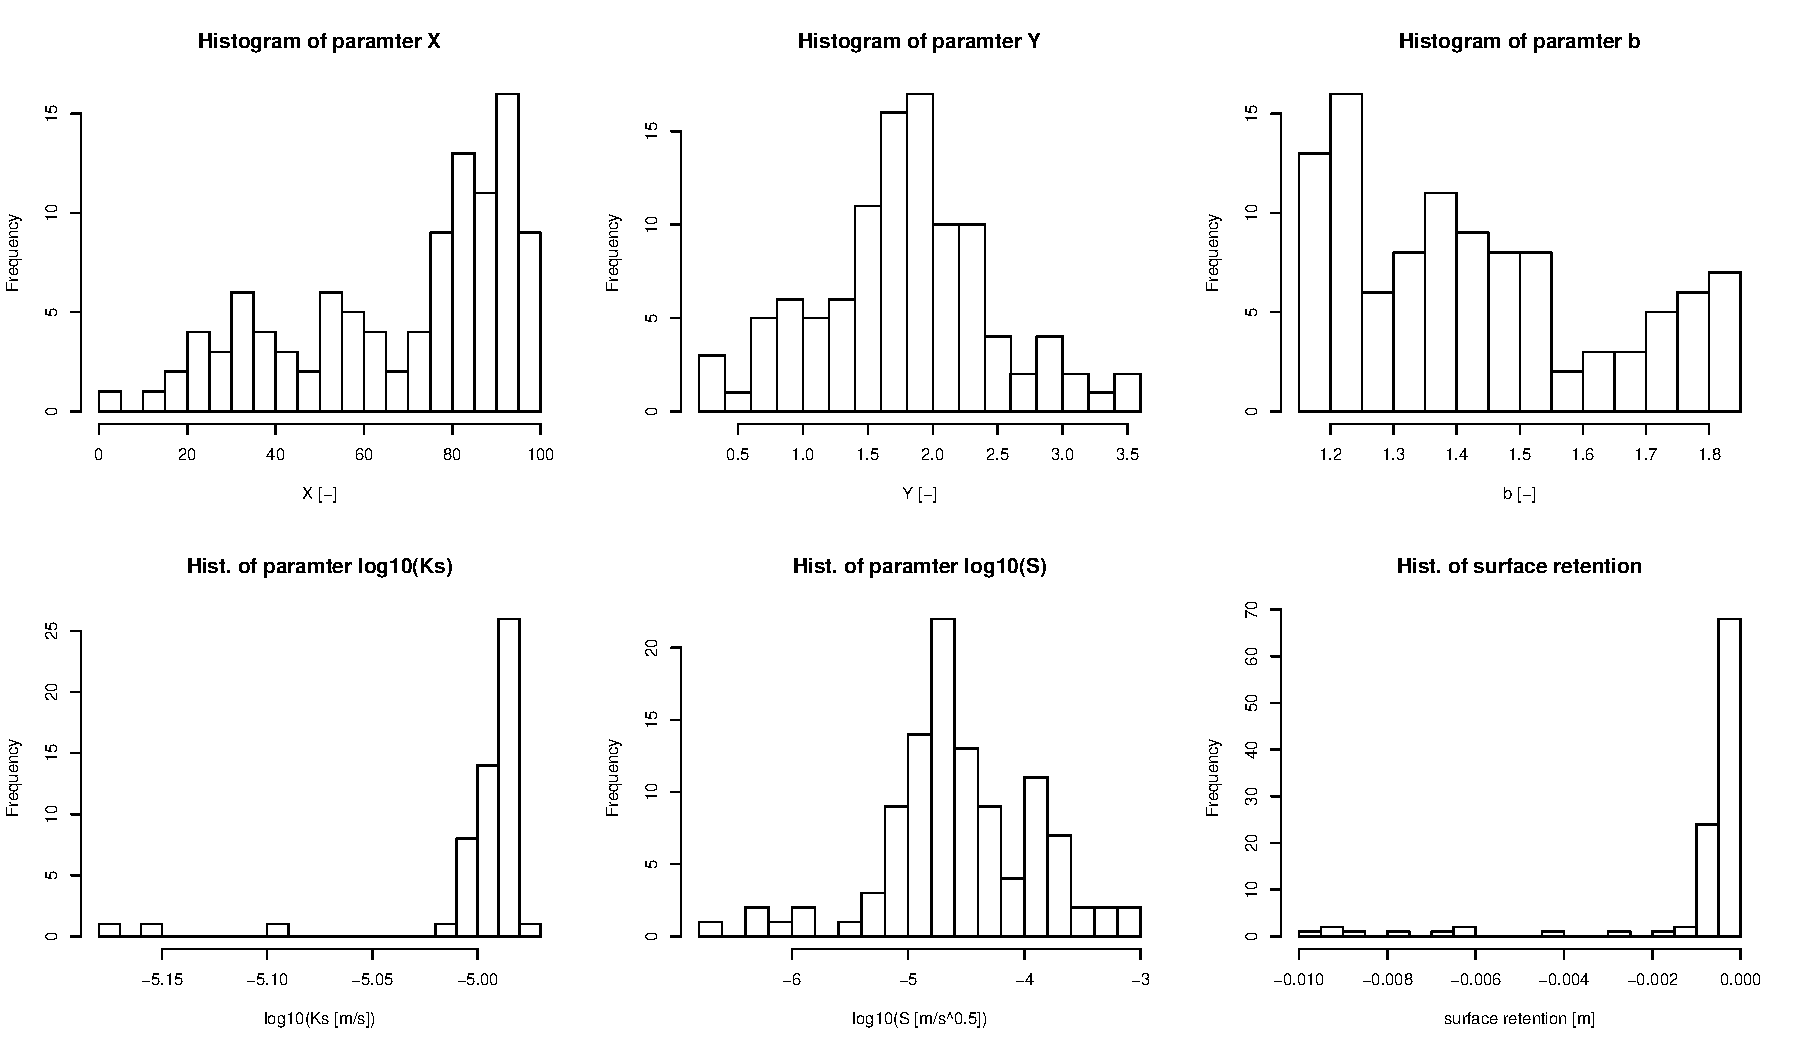
\includegraphics[width=0.7\paperwidth]{img/hystogram}
   \end{center}
\end{frame}


